% Paste these paragraphs into the existing team report under the matching headings.
% Confirm the actual hours and team totals before exporting the report.

% In Iteration 2 Table 4, change Olu's completed points from -- to 6.
% If the other rows are still Sam 5, Miles 7, and Cheick 6, change Total from 18 to 24.

% Add under the Iteration 2 retrospective, after the other personal reflections.
\paragraph{Olu's reflection}
In Iteration 2, I completed my assigned user-facing stories, but I did not update my row in the team speed table or add my reflection. That made the report incomplete even though the code was present. I learned that a working feature and its documentation need to be finished together. For this iteration I checked the story list, test results, diagram, and report text before calling my work complete.

% Add to the Iteration 3 Planning section.
\paragraph{Olu's plan}
I planned S14 (table chat, 5 points), S16 (spectate a table, 2 points), S19 (track wins and losses, 3 points), S36 (review game history, 5 points), S37 (leave a table, 2 points), and S39 (configure starting bots, 3 points), for a total of 20 points. These stories connect to the shared table and the player's profile. I focused on keeping the new screens and routes consistent with the existing game.

% Add to the Iteration 3 Work Done section.
\paragraph{Olu -- Table Chat, Spectating, Records, and Table Controls}
\begin{itemize}
    \item \textbf{S14 -- Table Chat (5 points):} Added messages for seated, connected players. The server saves messages by table and returns them in order. Empty and oversized messages are rejected.
    \item \textbf{S16 -- Spectate Table (2 points):} Added a watch link and a spectator page. Spectators can see the public state of a hand without taking a seat. Private tables ask for a password, and hidden player cards are not returned.
    \item \textbf{S19 -- Track Wins and Losses (3 points):} Added profile totals for saved hands, wins, losses, ties, win rate, and net chips. The totals come from the signed-in player's saved game results.
    \item \textbf{S36 -- Review My Game History (5 points):} Added a paged history of the player's hands with date filters and a session view opened from any hand. The server checks the signed-in account so one player cannot request another player's history.
    \item \textbf{S37 -- Leave Table (2 points):} Added a leave action that frees the seat after the current hand settles. The table keeps the player's remaining table chips for a later rejoin. This follows the game's current separate table-chip balance; the team should confirm whether the story instead requires a transfer to account chips.
    \item \textbf{S39 -- Configure Table Bots (3 points):} Added a starting-bot count to table creation, with validation that leaves room for a human host. Bots join the table through the existing shared game rules.
\end{itemize}
The implementation is on \texttt{feature/olu-iteration-3} and is awaiting team review. Actual time spent: S14 [confirm] hours; S16 [confirm] hours; S19 [confirm] hours; S36 [confirm] hours; S37 [confirm] hours; S39 [confirm] hours. Count these points as delivered in the team report only after the team accepts the work and merges it.

% Add to the Iteration 3 Testing Coverage section.
\paragraph{Olu's testing}
The server and client production builds pass. The server coverage command passed 358 tests with PostgreSQL enabled; the separate multiplayer acceptance test also passed. The client coverage command passed 113 tests. Coverage reports generated by the project tools show 93.12\% server statement coverage and 76.92\% client statement coverage, with 88.47\% and 83.30\% branch coverage respectively. Counting all covered statements together gives 81.62\% coverage, while combined branch coverage is 85.72\%. These exceed the assignment's coverage targets. The JSON coverage summaries are included under \texttt{Docs/}.

\begin{table}[H]
    \centering
    \begin{tabular}{|l|r|r|}
        \hline
        \textbf{Code} & \textbf{Statements} & \textbf{Branches} \\ \hline
        Server & 93.12\% & 88.47\% \\ \hline
        Client & 76.92\% & 83.30\% \\ \hline
        Combined by item count & 81.62\% & 85.72\% \\ \hline
    \end{tabular}
    \caption{Iteration 3 automated code coverage}
    \label{tab:iteration3-coverage}
\end{table}

% Add under the Iteration 3 retrospective and reflection.
\paragraph{Olu's reflection}
The main challenge was making several stories work with one shared table state. Leaving during a hand could remove a player too early, and a spectator response could accidentally expose private cards. I used the existing table service and added checks around those transitions, then ran the multiplayer test with PostgreSQL to check the full flow. I learned that a successful screen test does not prove that the same action works when several players are connected. Next time I would agree on the table-chip rule with the team before implementing leave and rejoin, and update the Kanban card and report as each story is tested.

% Upload iteration-3-gameplay-class-diagram.png to Overleaf and add this under System Design / Diagrams.
\begin{figure}[H]
    \centering
    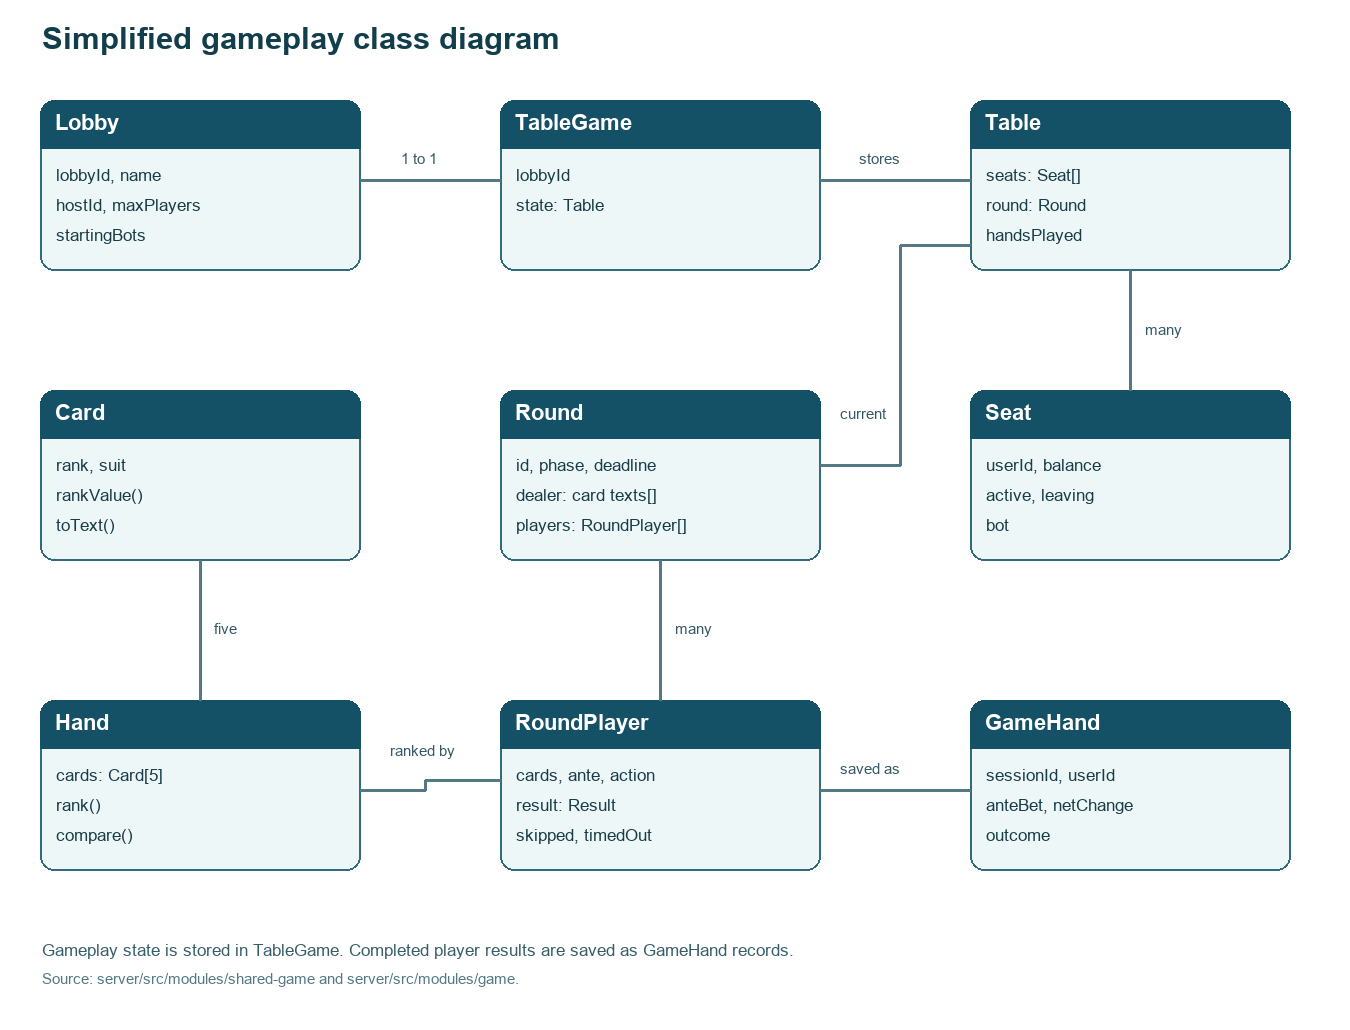
\includegraphics[width=0.9\textwidth]{iteration-3-gameplay-class-diagram.png}
    \caption{Simplified classes used by the shared gameplay flow}
    \label{fig:iteration3-gameplay-classes}
\end{figure}
